\documentclass{beamer}
\usepackage{amsmath,amssymb,amsthm}
\usepackage{algorithm,algorithmic}

\usepackage{tikz}
\usetikzlibrary{arrows,shapes,chains,matrix,positioning,scopes,patterns}
\usepackage{pgfplots}
\usepgflibrary{shapes}
\pgfplotsset{compat=1.6}

\usetheme{default}
\setbeamertemplate{navigation symbols}{\textcolor{blue}{\insertframenumber / \inserttotalframenumber}}

\newcommand{\expt}{\mathbb{E}}
\newcommand{\indicator}[1]{\mathbbm{1}_{\left\{ {#1} \right\} }}
\newcommand{\abs}[1]{\left\lvert#1\right\rvert}

\newlength\tikzwidth
\newlength\tikzheight

\title{\large{Spatially-Coupled Codes for Write-Once Memories}}
\author{\normalsize{\textbf{Santhosh Kumar} \\ Avinash Vem \\ Krishna Narayanan \\ Henry Pfister}}
\date{Allerton 2015}

\begin{document}

\begin{frame}
  \titlepage
\end{frame}

\begin{frame}{Write-Once Memories}
  \begin{center}
    \scalebox{0.5}{\begin{tikzpicture}
  [draw=black,thick, >=stealth']
  \foreach \x in {0,2cm,4cm,6cm,8cm,10cm,12cm,14cm,16cm} {
    \draw (\x,0) rectangle (\x+2cm,-1.5cm);
  }

  \only<3>{
    \foreach \x in {2cm,4cm,10cm,14cm} {
      \draw[fill=black] (\x,0) rectangle (\x+2cm,-1.5cm);
    }
  }

  \only<1>{
    \foreach \x in {0,2cm,4cm,6cm,8cm,10cm,12cm,14cm,16cm} {
      \node[white] at (\x+1cm,-2cm) {\Huge{$0$}};
    }
  }

  \only<2>{
    \foreach \x in {0,2cm,4cm,6cm,8cm,10cm,12cm,14cm,16cm} {
      \node[] at (\x+1cm,-2cm) {\Huge{$0$}};
    }
  }

  \only<3>{
    \foreach \x in {0,6cm,8cm,12cm,16cm} {
      \node[] at (\x+1cm,-2cm) {\Huge{$0$}};
    }

    \foreach \x in {2cm,4cm,10cm,14cm} {
      \node[red] at (\x+1cm,-2cm) {\Huge{$1$}};
    }
  }


%  \node[blue] at (3cm,-0.75cm) {$i$}; \node[blue] at (15cm,-0.75cm) {$j$};
%  \draw[->,thick] (5cm,-2cm) ..controls(11cm,-2.5cm) .. node[midway,below]{$\pi$} (17cm,-2cm);
\end{tikzpicture}


%%% Local Variables: 
%%% mode: latex
%%% TeX-master: "../talk"
%%% End: 
}    
  \end{center}
  \begin{block}{Flash Memory}<1->
    \begin{itemize}
    \item In typical flash memory, changing from $0$ to $1$ is easy
    \item Resetting $1$ to $0$ requires \textcolor{blue}{rewriting whole block}
    \item Write-once memories model such storage systems
    \end{itemize}
  \end{block}
  \begin{block}{Binary Write-Once Memories}<2->
    \begin{itemize}
    \item<2-> \textcolor{blue}{$0 \longrightarrow 1$ is allowed}
    \item<3-> \alert{$1 \longrightarrow 0$ is forbidden}
    \end{itemize}
  \end{block}
\end{frame}

\begin{frame}{Capacity Region (I) - Noiseless}
  \begin{center}
    \scalebox{0.5}{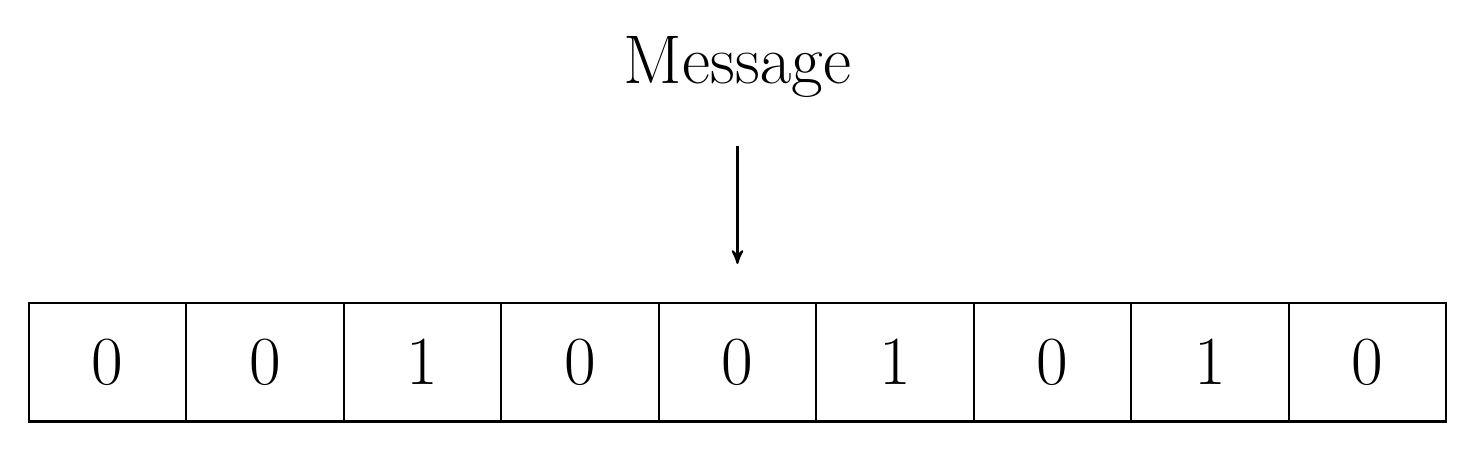
\begin{tikzpicture}
  [draw=black,thick, >=stealth']
  \foreach \x in {0,2cm,4cm,6cm,8cm,10cm,12cm,14cm,16cm} {
    \draw (\x,0) rectangle (\x+2cm,-1.5cm);
  }

  \foreach \x in {0,2cm,6cm,8cm,12cm,16cm} {
    \node[] at (\x+1cm,-0.75cm) {\Huge{$0$}};
  }

  \foreach \x in {4cm,10cm,14cm} {
    \node[] at (\x+1cm,-0.75cm) {\Huge{$1$}};
  }

  \node at (9cm,3cm) {\Huge{Message}};

  \draw[->] (9cm,2cm) -- (9cm,0.5cm);

\end{tikzpicture}



%%% Local Variables: 
%%% mode: latex
%%% TeX-master: "../talk"
%%% End: 
}    
  \end{center}
  \begin{block}{Write-Once Memory without Noise}
    \begin{itemize}
    \item In 1982, Rivest and Shamir gave first WOM codes 
      \begin{itemize}
      \item 2 bits in 2 writes with only 3 cells
      \end{itemize}
    \item Only about \textcolor{blue}{$n t / \log(t)$ cells} required to store $n$ bits for $t$ writes
    \item<2-> In 1985, Heegard gave the \alert{capacity} for $t$-write system
    \item<2-> For a $2$-write system, it is
      \begin{align*}
        & \Big{\{} (R_1,R_2) \mid 0 \leq R_1 <  h(\delta) , \,\,0 \leq R_2 < 1-\delta \Big{\}} 
      \end{align*}
    \end{itemize}
  \end{block}
\end{frame}

\begin{frame}{Capacity Region (II) - Read Errors}
  \begin{center}
    \scalebox{0.5}{\input{Figures/write-once-memory-capacity-noisy}}
  \end{center}
  \begin{block}{Write-Once Memory with Read Errors}
    \begin{itemize}
    \item Different from write errors
    \item $Y = X \oplus \mathsf{Ber}(p)$, where $\mathsf{Ber}(p)$ denotes the Bernoulli noise
    \item Capacity region is \alert{unknown}
    \end{itemize}
  \end{block}
\end{frame}

\begin{frame}{Main Result}
  \begin{block}{Objective}<1->
    \begin{itemize}
    \item Construct \alert{low-complexity} coding schemes that achieve the \textcolor{blue}{capacity region} of the WOM system\vspace{0.1cm}
      \begin{itemize}
      \item<1-> Low-complexity encoding and decoding
      \end{itemize}
    \item<2-> Focus on the 2-write WOM system
      \begin{itemize}
      \item Achieves the capacity region of the noiseless system
      \item For read errors, achieves
        \begin{align*}
          R_1 &< h(\delta) - h(p), & R_2 &< 1 - \delta - h(p) .
        \end{align*}
      \end{itemize}
    \item<3-> Extension to multi-write systems \alert{seems possible with BPGD}
    \end{itemize}
  \end{block}
  \begin{block}{Idea}<4->
    \begin{itemize}
      \item Use compound LDGM/LDPC codes
      \item Encoding for second write is \alert{erasure quantization}
      \item Use \textcolor{blue}{spatial coupling with message-passing}
    \end{itemize}
  \end{block}
\end{frame}

\begin{frame}{Compound LDGM/LDPC Codes}
  \begin{columns}
    \column{0.45\textwidth}
    \begin{center}
      \setlength\tikzheight{5cm}
      \setlength\tikzwidth{6cm}
      \scalebox{0.5}{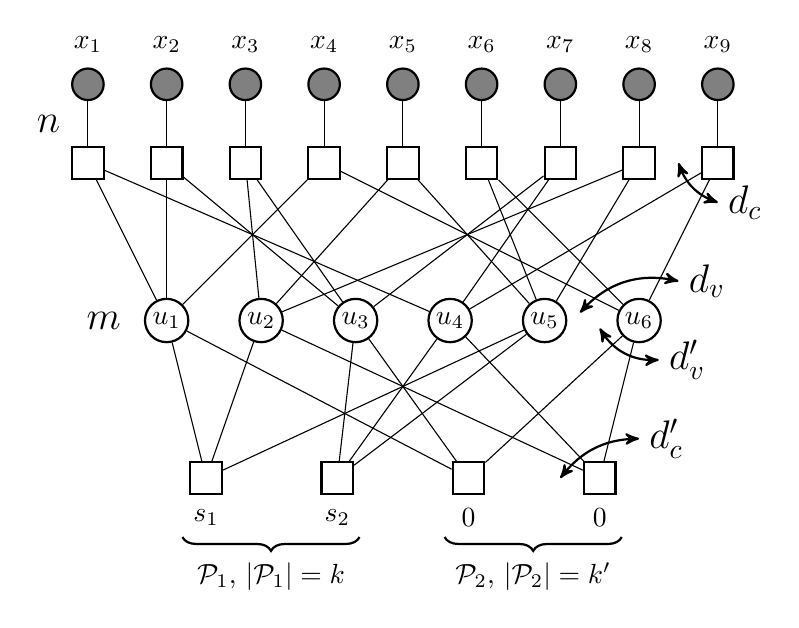
\begin{tikzpicture}
  [
  node distance = 12mm, draw=black, thick, >=stealth',
  bitnode/.style={circle, inner sep = 0pt, minimum size = 5.5mm, draw=black},
  checknode/.style={rectangle, inner sep = 0pt, minimum size = 4mm, draw=black},
  bitnode2/.style={circle, inner sep = 0pt, minimum size = 4mm, draw=black, fill=black!50},
  ]
  
  \foreach \x in {1,2,...,9} {
    \node[bitnode2] (bb\x) at (\x-5,3) {};
  }

  \foreach \y in {1,2,...,9} {
    \node at (\y-5,3.5) {$x_{\y}$};
  }

  \foreach \x in {1,2,...,9} {
    \node[checknode] (c\x) at (\x-5,2) {};
    \draw[thin] (c\x) -- (bb\x);
  }

  \foreach \x in {1,2,...,6} {
    \node[bitnode] (b\x) at (1.2*\x-4.2,0) {$u_{\x}$};
  }

  \foreach \x in {1,...,4} {
    \node[checknode] (cc\x) at (5*\x/3-2.5-5/3,-2) {};
  }

  \draw[thin] (c1) -- (b4);
  \draw[thin] (c1) -- (b1);
  \draw[thin] (c2) -- (b1);
  \draw[thin] (c2) -- (b3);
  \draw[thin] (c3) -- (b3);
  \draw[thin] (c3) -- (b2);
  \draw[thin] (c4) -- (b1);
  \draw[thin] (c4) -- (b6);
  \draw[thin] (c5) -- (b2);
  \draw[thin] (c5) -- (b5);
  \draw[thin] (c6) -- (b5);
  \draw[thin] (c6) -- (b6);
  \draw[thin] (c7) -- (b3);
  \draw[thin] (c7) -- (b4);
  \draw[thin] (c8) -- (b5);
  \draw[thin] (c8) -- (b2);
  \draw[thin] (c9) -- (b4);
  \draw[thin] (c9) -- (b6);


  \draw[thin] (cc1) -- (b2);
  \draw[thin] (cc1) -- (b1);
  \draw[thin] (cc1) -- (b5);
  \draw[thin] (cc2) -- (b5);
  \draw[thin] (cc2) -- (b3);
  \draw[thin] (cc2) -- (b4);
  \draw[thin] (cc3) -- (b1);
  \draw[thin] (cc3) -- (b3);
  \draw[thin] (cc3) -- (b6);
  \draw[thin] (cc4) -- (b2);
  \draw[thin] (cc4) -- (b6);
  \draw[thin] (cc4) -- (b4);

  \draw[<->] (3.5,2) to [bend right=25] (4,1.5) node [right] {\Large $d_{c}$};
  \draw[<->] (2.25,0.1) to [bend left=30] (3.5,0.5) node [right] {\Large $d_{v}$};
  \draw[<->] (2.5,-0.1) to [bend right=30] (3.25,-0.5) node [right] {\Large $d'_{v}$};
  \draw[<->] (2,-2) to [bend left=25] (3,-1.5) node [right] {\Large $d'_{c}$};

  \node at (-4.5,2.5) {\Large $n$};
  \node at (-3.8,0) {\Large $m$};

  \node at (5*1/3-2.5-5/3,-2.5) {$s_1$};
  \node at (5*2/3-2.5-5/3,-2.5) {$s_2$};
  \node at (5*3/3-2.5-5/3,-2.5) {$0$};
  \node at (5*4/3-2.5-5/3,-2.5) {$0$};

  \draw[decorate,decoration={brace,amplitude=5pt,mirror}] (-2.8,-2.75) -- (-0.55,-2.75) node [midway,yshift=-0.5cm] {$\mathcal{P}_1$,  $|\mathcal{P}_1|=k$};
  \draw[decorate,decoration={brace,amplitude=5pt,mirror}] (3.33-2.8,-2.75) -- (3.33-0.55,-2.75) node [midway,yshift=-0.5cm]{$\mathcal{P}_2$,  $|\mathcal{P}_2|=k'$};
\end{tikzpicture}

%%% Local Variables: 
%%% mode: latex
%%% TeX-master: "../isit14"
%%% End: 
}
    \end{center}
    \column{0.55\textwidth}
    \begin{itemize}
    \item Codebook $(n,m-k-k')$ \vspace{0.1cm}
    \item \textcolor{blue}{Message constraints} \vspace{-0.2cm}
      \begin{align*}
        u_1\oplus u_2 \oplus u_5&=s_1, &  u_1\oplus u_3 \oplus u_6&=0
      \end{align*}
    \item Codeword $(x_1,\cdots,x_9)$: \vspace{-0.2cm}
      \begin{align*}
        x_1 &= u_1 \oplus u_4, & x_2 &= \cdots
      \end{align*}
    \item Parametrized by $s^k$: $\mathcal{C}(s^k)$
    \end{itemize}
  \end{columns}
  \vspace{0.2cm}
  \begin{block}{Key Properties of Compound Codes}<2->
      \begin{itemize}
      \item a natural \textcolor{red}{coset decomposition}: $\mathcal{C}=\bigcup_{s^k \in \{0,1\}^k} \mathcal{C}(s^k)$
      \item achieves capacity over eras. chan. under MAP (when $m=n$)
      \item a \textcolor{blue}{good source code} under optimal encoding
      \item a \textcolor{blue}{good channel code} under optimal decoding
      \end{itemize}
  \end{block}
\end{frame}

\begin{frame}{Good Code}
  \begin{block}{``Good'' source code}
    \begin{itemize}
    \item Rate of the code is $R=1-h(\delta)+\varepsilon$
    \item When this code is used to \alert{optimally encode} $\mathsf{Ber}(\tfrac{1}{2})$
    \item The average Hamming \textcolor{blue}{distortion is at most $\delta$}
    \end{itemize}
  \end{block}
  \vspace{0.4cm}
  \begin{block}{``Good'' channel code}
    \begin{itemize}
    \item Rate of the code is $R=1-h(p)-\varepsilon$
    \item When this code is used for channel coding on $\mathsf{BSC}(p)$
    \item Message est.~under \alert{optimal decoding} with \textcolor{blue}{error at most $\varepsilon$}
    \end{itemize}
  \end{block}
\end{frame}

\begin{frame}{Coding Scheme for 2-write WOM: First Write}
  \vspace{-2cm}
  \begin{center}
    \begin{align*}
      R_1 < h(\delta) - h(p)
    \end{align*}
  \end{center}
  \vspace{-0.5cm}
  \begin{columns}
    \column{0.45\textwidth}
    \begin{center}
      \scalebox{0.5}{\input{Figures/coding-scheme-first-write}}
    \end{center}

    \column{0.45\textwidth}
    \begin{itemize}
    \item<1-> With message $s^k$, encode $0^n$ to $x^n$ (Distortion $\approx \delta$)
    \item<1-> \textcolor{red}{Store $x^n$}
    \item<2-> Decoder has
      \small{
        \begin{align*}
          y_i&=x_i \oplus \mathsf{Ber}(p) \\
        \end{align*}
      }
    \vspace{-1.25cm}
    \item <3-> \textcolor{blue}{Dec. $x^n$ and compute $s^k$}
    \item <3-> $R_1=\tfrac{k}{n}\approx h(\delta)-h(p)$
    \end{itemize}
  \end{columns}
\end{frame}

\begin{frame}{Coding Scheme for 2-write WOM: Second Write}
  \begin{center}
    \scalebox{0.5}{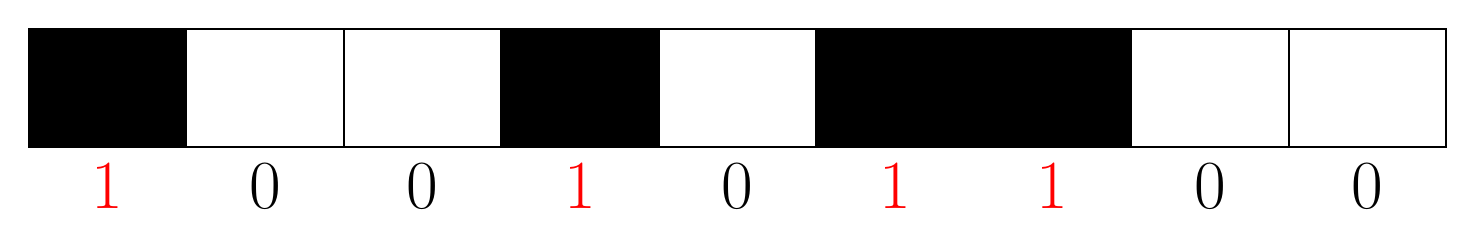
\begin{tikzpicture}
  [draw=black,thick, >=stealth']
  \foreach \x in {0,2cm,4cm,6cm,8cm,10cm,12cm,14cm,16cm} {
    \draw (\x,0) rectangle (\x+2cm,-1.5cm);
  }

  \foreach \x in {0,6cm,10cm,12cm} {
    \draw[fill=black] (\x,0) rectangle (\x+2cm,-1.5cm);
  }
  
  \foreach \x in {2cm,4cm,8cm,14cm,16cm} {
    \node[] at (\x+1cm,-2cm) {\Huge{$0$}};
  }
  
  \foreach \x in {0,6cm,10cm,12cm} {
    \node[red] at (\x+1cm,-2cm) {\Huge{$1$}};
  }
  

\end{tikzpicture}

%%% Local Variables: 
%%% mode: latex
%%% TeX-master: "../talk"
%%% End: 
}    
  \end{center}
  \begin{columns}
    \column{0.45\textwidth}
    \begin{center}
      \scalebox{0.55}{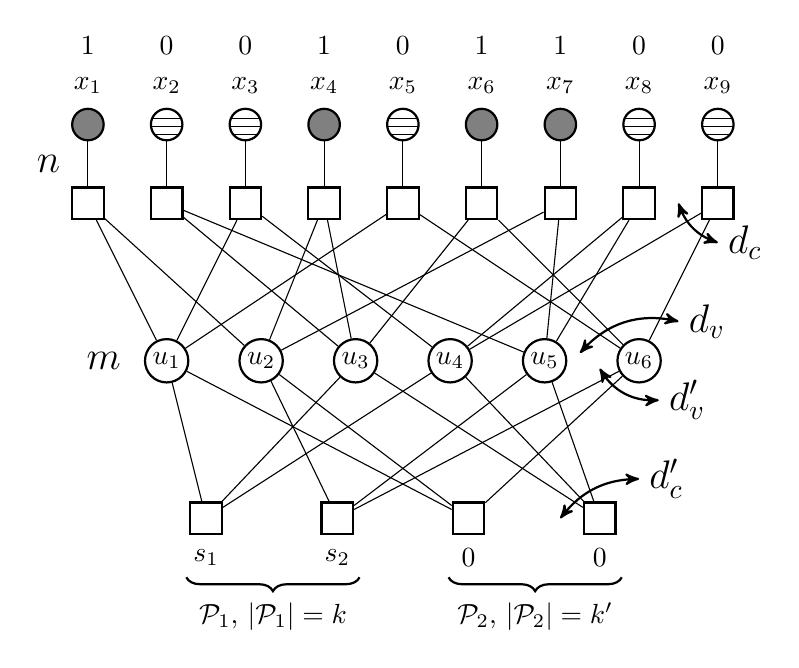
\begin{tikzpicture}
  [
  node distance = 12mm, draw=black, thick, >=stealth',
  ldpc_bitnode/.style={circle, inner sep = 0pt, minimum size = 5.5mm, draw=black},
  checknode/.style={rectangle, inner sep = 0pt, minimum size = 4mm, draw=black},
  ldgm_bitnode/.style={circle, inner sep = 0pt, minimum size = 4mm, draw=black},
  ]
  
  \node[ldgm_bitnode,fill=black!50] (ldgmb1) at (1-5,3) {}; \node at (1-5,4) {$1$};
  \node[ldgm_bitnode,pattern=horizontal lines] (ldgmb2) at (2-5,3) {}; \node at (2-5,4) {$0$};
  \node[ldgm_bitnode,pattern=horizontal lines] (ldgmb3) at (3-5,3) {}; \node at (3-5,4) {$0$};
  \node[ldgm_bitnode,fill=black!50] (ldgmb4) at (4-5,3) {}; \node at (4-5,4) {$1$};
  \node[ldgm_bitnode,pattern=horizontal lines] (ldgmb5) at (5-5,3) {}; \node at (5-5,4) {$0$};
  \node[ldgm_bitnode,fill=black!50] (ldgmb6) at (6-5,3) {}; \node at (6-5,4) {$1$};
  \node[ldgm_bitnode,fill=black!50] (ldgmb7) at (7-5,3) {}; \node at (7-5,4) {$1$};
  \node[ldgm_bitnode,pattern=horizontal lines] (ldgmb8) at (8-5,3) {}; \node at (8-5,4) {$0$};
  \node[ldgm_bitnode,pattern=horizontal lines] (ldgmb9) at (9-5,3) {}; \node at (9-5,4) {$0$};

  \foreach \y in {1,2,...,9} {
    \node at (\y-5,3.5) {$x_{\y}$};
  }

  \foreach \x in {1,2,...,9} {
    \node[checknode] (ldgmc\x) at (\x-5,2) {};
    \draw[thin] (ldgmc\x) -- (ldgmb\x);
  }

  \foreach \x in {1,2,...,6} {
    \node[ldpc_bitnode] (ldpcb\x) at (1.2*\x-4.2,0) {$u_{\x}$};
  }

  \foreach \x in {1,...,4} {
    \node[checknode] (ldpcc\x) at (5*\x/3-2.5-5/3,-2) {};
  }

  \draw[thin] (ldpcb1) -- (ldgmc3);
  \draw[thin] (ldpcb1) -- (ldgmc1);
  \draw[thin] (ldpcb1) -- (ldgmc5);
  \draw[thin] (ldpcb2) -- (ldgmc1);
  \draw[thin] (ldpcb2) -- (ldgmc7);
  \draw[thin] (ldpcb2) -- (ldgmc4);
  \draw[thin] (ldpcb3) -- (ldgmc4);
  \draw[thin] (ldpcb3) -- (ldgmc6);
  \draw[thin] (ldpcb3) -- (ldgmc2);
  \draw[thin] (ldpcb4) -- (ldgmc3);
  \draw[thin] (ldpcb4) -- (ldgmc8);
  \draw[thin] (ldpcb4) -- (ldgmc9);
  \draw[thin] (ldpcb5) -- (ldgmc7);
  \draw[thin] (ldpcb5) -- (ldgmc8);
  \draw[thin] (ldpcb5) -- (ldgmc2);
  \draw[thin] (ldpcb6) -- (ldgmc6);
  \draw[thin] (ldpcb6) -- (ldgmc5);
  \draw[thin] (ldpcb6) -- (ldgmc9);


  \draw[thin] (ldpcc1) -- (ldpcb4);
  \draw[thin] (ldpcc1) -- (ldpcb1);
  \draw[thin] (ldpcc1) -- (ldpcb3);
  \draw[thin] (ldpcc2) -- (ldpcb5);
  \draw[thin] (ldpcc2) -- (ldpcb2);
  \draw[thin] (ldpcc2) -- (ldpcb6);
  \draw[thin] (ldpcc3) -- (ldpcb2);
  \draw[thin] (ldpcc3) -- (ldpcb6);
  \draw[thin] (ldpcc3) -- (ldpcb1);
  \draw[thin] (ldpcc4) -- (ldpcb3);
  \draw[thin] (ldpcc4) -- (ldpcb5);
  \draw[thin] (ldpcc4) -- (ldpcb4);

  \draw[<->] (3.5,2) to [bend right=25] (4,1.5) node [right] {\Large $d_{c}$};
  \draw[<->] (2.25,0.1) to [bend left=30] (3.5,0.5) node [right] {\Large $d_{v}$};
  \draw[<->] (2.5,-0.1) to [bend right=30] (3.25,-0.5) node [right] {\Large $d'_{v}$};
  \draw[<->] (2,-2) to [bend left=25] (3,-1.5) node [right] {\Large $d'_{c}$};

  \node at (-4.5,2.5) {\Large $n$};
  \node at (-3.8,0) {\Large $m$};

  \node at (5*1/3-2.5-5/3,-2.5) {$s_1$};
  \node at (5*2/3-2.5-5/3,-2.5) {$s_2$};
  \node at (5*3/3-2.5-5/3,-2.5) {$0$};
  \node at (5*4/3-2.5-5/3,-2.5) {$0$};

  \draw[decorate,decoration={amplitude=5pt,mirror,brace}] (-2.75,-2.75) -- (-0.55,-2.75) node [yshift=-0.5cm,midway] {$\mathcal{P}_1$,  $|\mathcal{P}_1|=k$};
  \draw[decorate,decoration={amplitude=5pt,mirror,brace}] (3.33-2.75,-2.75) -- (3.33-0.55,-2.75) node [yshift=-0.5cm,midway]{$\mathcal{P}_2$,  $|\mathcal{P}_2|=k'$};

\end{tikzpicture}

%%% Local Variables: 
%%% mode: latex
%%% TeX-master: "../paper"
%%% End: 
}
    \end{center}
    \column{0.45\textwidth}
    \begin{itemize}
    \item Need to find a \alert{consistent} codeword in $\mathcal{C}(s^k)$
    \item<2-> Closely related to \textcolor{blue}{Binary Erasure Quantization (BEQ)}
    \item<2-> En Gad, Huang, Li and Bruck (ISIT 2015)
    \end{itemize}
  \end{columns}
\end{frame}

\begin{frame}{Binary Erasure Quantization}
  \begin{itemize}
  \item Quantize a sequence in $\{0,1,*\}^n$ to $x^n \in \mathcal{C} \subset \{0,1\}^n$
    \begin{itemize}
    \item $0$'s and $1$'s should \alert{match exactly}
    \item $*$'s can take \textcolor{blue}{either $0$ or $1$}
    \end{itemize}
    \vspace{0.25cm}
  \item Can map the second write of 2-write WOM to BEQ
    \begin{itemize}
    \item Map $0$'s to $*$'s and keep $1$'s
    \item Quantize to codeword in $\mathcal{C}(s^k)$
    \end{itemize}
\vspace{0.25cm}
  \item BEQ is the dual of decoding on binary erasure channel
    \begin{itemize}
    \item Martinian and Yedidia (Allerton 2003)
    \item Can quan. all seq. with erasure pattern $e^n \in \{0,1\}^n$ to $\mathcal{C}$ \\ \hspace{3.5cm} $\Updownarrow$ \\ Chan. dec. for $\mathcal{C}^{\perp}$ can correct all vectors with eras. $1^n \oplus e^n$
    \end{itemize}
    \vspace{0.25cm}
  \item Choose a good (dual) code $\mathcal{C}(s^k)$
  \end{itemize}
\end{frame}

\begin{frame}{Coding Scheme for 2-write WOM: Second Write}
  \vspace{-2cm}
  \begin{center}
    \begin{align*}
      R_2 < 1 - \delta - h(p)
    \end{align*}
  \end{center}
  \vspace{-0.5cm}
  \begin{columns}
    \column{0.45\textwidth}
    \begin{center}
      \scalebox{0.5}{\input{Figures/coding-scheme-second-write}}
    \end{center}

    \column{0.45\textwidth}
    \begin{itemize}
    \item<1-> \alert{Change $0$'s to $*$'s}
    \item<1-> With message $s^k$, encode seq. to $\mathcal{C}(s^k)$
    \item<2-> Decoder has
      \small{
        \begin{align*}
          y_i&=x_i \oplus \mathsf{Ber}(p) \\
        \end{align*}
      }
    \vspace{-1.25cm}
    \item <3-> \textcolor{blue}{Dec. $x^n$ and compute $s^k$}
    \item <3-> $R_2=\tfrac{k}{n}\approx 1 - \delta - h(p)$
    \end{itemize}
  \end{columns}
\end{frame}

\begin{frame}{Iterative Erasure Quantization Algorithm}
  \begin{center}
    \scalebox{0.5}{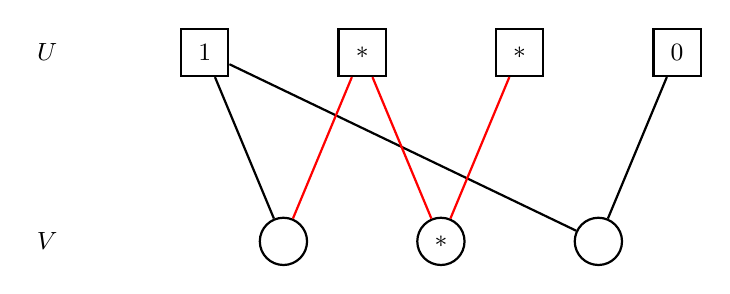
\begin{tikzpicture}
  [
  yscale=1.2,
  node distance = 12mm, draw=black, thick, >=stealth',
  bitnode/.style={circle, inner sep = 0pt, minimum size = 6mm, draw=black},
  checknode/.style={rectangle, inner sep = 0pt, minimum size = 6mm, draw=black},
  ]
  
  \node[checknode] (c1) at (1,2) {\small{$1$}};
  \node[checknode] (c2) at (3,2) {\small{$*$}};
  \node[checknode] (c3) at (5,2) {\small{$*$}};
  \node[checknode] (c4) at (7,2) {\small{$0$}};


  \node[bitnode] (b1) at (2,0) {};
  \node[bitnode] (b2) at (4,0) {\small{$*$}};
  \node[bitnode] (b3) at (6,0) {};

  \draw[thick] (c1) -- (b1);
  \draw[thick] (c1) -- (b3);
  \draw[thick,red] (c2) -- (b1);
  \draw[thick,red] (c2) -- (b2);
  \draw[thick,red] (c3) -- (b2);
  \draw[thick] (c4) -- (b3);

  \node at (-1,2) {\small{$U$}};
  \node at (-1,0) {\small{$V$}};


\end{tikzpicture}

%%% Local Variables: 
%%% mode: latex
%%% TeX-master: "../talk"
%%% End: 
}
  \end{center}
  \begin{itemize}
  \item \alert{Peeling type encoder}
  \begin{center}
    \begin{algorithmic}
      \WHILE{$\exists$ non-erasures in $V$}
      \IF{$\exists$ non-erased $u \in U$ such that only one of its neighbors $v \in V$ is not erased}
      \STATE Pair $(u,v)$.
      \STATE Erase $u$ and $v$.
      \ELSE
      \STATE FAIL.
      \STATE \textbf{break}.
      \ENDIF
      \ENDWHILE
    \end{algorithmic}
  \end{center}

  \end{itemize}
\end{frame}

\begin{frame}{Remarks}
  \begin{itemize}
  \item Need codes that are \alert{simultaneously good} for channel/source coding and erasure quantization \vspace{0.2cm}
  \item Use \textcolor{blue}{message-passing algorithms} instead of \alert{optimal} \vspace{0.2cm}
  \item Use spatial-coupling for \alert{goodness} of codes under message-passing \vspace{0.2cm}
  \end{itemize}
\end{frame}

\begin{frame}{Spatially-Coupled Compound LDGM/LDPC Codes}
  \begin{center}
    \scalebox{0.7}{\begin{tikzpicture}[
  xscale=0.33,yscale=1,
  bitnode/.style={circle,minimum size=10pt,thick,draw=black,fill=white},
  bitnodeblack/.style={circle,minimum size=10pt,thick,draw=black,fill=white},
  bitnodewhite/.style={circle,minimum size=10pt,thick,draw=white,fill=white},
  bitnode2/.style={circle,minimum size=10pt,thick,draw=black,fill=gray},
  bitnode2black/.style={circle,minimum size=10pt,thick,draw=black,fill=gray},
  bitnode2white/.style={circle,minimum size=10pt,thick,draw=white,fill=white},
  checknode/.style={rectangle,minimum size=8pt,thick,draw=black,fill=white},
  checknodeblack/.style={rectangle,minimum size=8pt,thick,draw=black,fill=white},
  checknodewhite/.style={rectangle,minimum size=8pt,thick,draw=white,fill=white},
  permnode/.style={rectangle,very thin,minimum width=30pt,minimum height=18pt,fill=white,draw=black},
  permnodeblack/.style={rectangle,very thin,minimum width=30pt,minimum height=18pt,fill=white,draw=black},
  permnodewhite/.style={rectangle,very thin,minimum width=30pt,minimum height=18pt,fill=white,draw=white},
  permedge/.style={black!65},
  permedgeblack/.style={black!65},
  permedgewhite/.style={white},
  ]

  \def \cndist {0.75}
  \def \vndist {0.75}
  \def \ccndist {0.75}
  \def \vvny {2.75}
  \def \cny {2}
  \def \vny {-2}
  \def \ccny {-6}

  \def \midx   {0.5}

  \only<1>{
    \foreach \x/\i/\col in {0/1/white,6/2/white,12/3/white,18/4/black,24/5/white,30/6/white,36/7/white} {
      \draw[\col] (\x-\cndist, \cny) +(0,0) -- +(240:1);
      \draw[\col] (\x-\cndist, \cny) +(0,0) -- +(255:1);
      \draw[\col] (\x-\cndist, \cny) +(0,0) -- +(270:1);
      \draw[\col] (\x-\cndist, \cny) +(0,0) -- +(285:1);
      \draw[\col] (\x-\cndist, \cny) +(0,0) -- +(300:1);

      \draw[\col] (\x+\cndist, \cny) +(0,0) -- +(240:1);
      \draw[\col] (\x+\cndist, \cny) +(0,0) -- +(255:1);
      \draw[\col] (\x+\cndist, \cny) +(0,0) -- +(270:1);
      \draw[\col] (\x+\cndist, \cny) +(0,0) -- +(285:1);
      \draw[\col] (\x+\cndist, \cny) +(0,0) -- +(300:1);

      \draw[\col] (\x-\vndist, \vny) +(0,0) -- +(52.5:1);
      \draw[\col] (\x-\vndist, \vny) +(0,0) -- +(67.5:1);
      \draw[\col] (\x-\vndist, \vny) +(0,0) -- +(82.5:1);
      \draw[\col] (\x-\vndist, \vny) +(0,0) -- +(97.5:1);
      \draw[\col] (\x-\vndist, \vny) +(0,0) -- +(112.5:1);
      \draw[\col] (\x-\vndist, \vny) +(0,0) -- +(127.5:1);

      \draw[\col] (\x+\vndist, \vny) +(0,0) -- +(52.5:1);
      \draw[\col] (\x+\vndist, \vny) +(0,0) -- +(67.5:1);
      \draw[\col] (\x+\vndist, \vny) +(0,0) -- +(82.5:1);
      \draw[\col] (\x+\vndist, \vny) +(0,0) -- +(97.5:1);
      \draw[\col] (\x+\vndist, \vny) +(0,0) -- +(112.5:1);
      \draw[\col] (\x+\vndist, \vny) +(0,0) -- +(127.5:1);

      \draw[\col] (\x-\vndist, \vny) +(0,0) -- +(240:1);
      \draw[\col] (\x-\vndist, \vny) +(0,0) -- +(255:1);
      \draw[\col] (\x-\vndist, \vny) +(0,0) -- +(270:1);
      \draw[\col] (\x-\vndist, \vny) +(0,0) -- +(285:1);
      \draw[\col] (\x-\vndist, \vny) +(0,0) -- +(300:1);

      \draw[\col] (\x+\vndist, \vny) +(0,0) -- +(240:1);
      \draw[\col] (\x+\vndist, \vny) +(0,0) -- +(255:1);
      \draw[\col] (\x+\vndist, \vny) +(0,0) -- +(270:1);
      \draw[\col] (\x+\vndist, \vny) +(0,0) -- +(285:1);
      \draw[\col] (\x+\vndist, \vny) +(0,0) -- +(300:1);

      \draw[\col] (\x-\vndist, \ccny) +(0,0) -- +(52.5:1);
      \draw[\col] (\x-\vndist, \ccny) +(0,0) -- +(67.5:1);
      \draw[\col] (\x-\vndist, \ccny) +(0,0) -- +(82.5:1);
      \draw[\col] (\x-\vndist, \ccny) +(0,0) -- +(97.5:1);
      \draw[\col] (\x-\vndist, \ccny) +(0,0) -- +(112.5:1);
      \draw[\col] (\x-\vndist, \ccny) +(0,0) -- +(127.5:1);

      \draw[\col] (\x+\vndist, \ccny) +(0,0) -- +(52.5:1);
      \draw[\col] (\x+\vndist, \ccny) +(0,0) -- +(67.5:1);
      \draw[\col] (\x+\vndist, \ccny) +(0,0) -- +(82.5:1);
      \draw[\col] (\x+\vndist, \ccny) +(0,0) -- +(97.5:1);
      \draw[\col] (\x+\vndist, \ccny) +(0,0) -- +(112.5:1);
      \draw[\col] (\x+\vndist, \ccny) +(0,0) -- +(127.5:1);

      \node[checknode\col] (c1\i) at (\x-\cndist, \cny) {};
      \node[checknode\col] (c2\i) at (\x+\cndist, \cny) {};
      \node[bitnode\col] (v1\i) at (\x-\vndist, \vny) {};
      \node[bitnode\col] (v2\i) at (\x+\vndist, \vny) {};
      \node[checknode\col] (cc1\i) at (\x-\ccndist, \ccny) {};
      \node[checknode\col] (cc2\i) at (\x+\ccndist, \ccny) {};

      \node[bitnode2\col] (vv1\i) at (\x-\cndist,\vvny) {};
      \node[bitnode2\col] (vv2\i) at (\x+\cndist,\vvny) {};
      \draw[\col] (vv1\i) -- (c1\i);
      \draw[\col] (vv2\i) -- (c2\i);

      \foreach \j in {-5.7,-2.3,-1.7,1.7} {
        \node[\col] at (\x,\j) {\tiny{$...$}};
      }

      \node[permnode\col] (perm1_node\i) at (\x,\cny-1) {\textcolor{\col}{\footnotesize{$\pi$}}};
      \node[permnode\col] (perm2_node\i) at (\x,\vny+1) {\textcolor{\col}{\footnotesize{$\pi$}}};   
      \node[permnode\col] (perm3_node\i) at (\x,\vny-1) {\textcolor{\col}{\footnotesize{$\pi$}}};
      \node[permnode\col] (perm4_node\i) at (\x,\ccny+1) {\textcolor{\col}{\footnotesize{$\pi$}}};

      \draw[permedge\col] (perm1_node\i) .. controls (\x-0.2,0) .. (perm2_node\i);
      \draw[permedge\col] (perm1_node\i) .. controls (\x+0.2,0) .. (perm2_node\i);
      \draw[permedge\col] (perm3_node\i) .. controls (\x-0.2,-4) .. (perm4_node\i);
      \draw[permedge\col] (perm3_node\i) .. controls (\x+0.2,-4) .. (perm4_node\i);
    }
  }

  \only<2>{
    \foreach \x/\i in {0/1,6/2,12/3,18/4,24/5,30/6,36/7} {
      \draw[] (\x-\cndist, \cny) +(0,0) -- +(240:1);
      \draw[] (\x-\cndist, \cny) +(0,0) -- +(255:1);
      \draw[] (\x-\cndist, \cny) +(0,0) -- +(270:1);
      \draw[] (\x-\cndist, \cny) +(0,0) -- +(285:1);
      \draw[] (\x-\cndist, \cny) +(0,0) -- +(300:1);

      \draw[] (\x+\cndist, \cny) +(0,0) -- +(240:1);
      \draw[] (\x+\cndist, \cny) +(0,0) -- +(255:1);
      \draw[] (\x+\cndist, \cny) +(0,0) -- +(270:1);
      \draw[] (\x+\cndist, \cny) +(0,0) -- +(285:1);
      \draw[] (\x+\cndist, \cny) +(0,0) -- +(300:1);

      \draw[] (\x-\vndist, \vny) +(0,0) -- +(52.5:1);
      \draw[] (\x-\vndist, \vny) +(0,0) -- +(67.5:1);
      \draw[] (\x-\vndist, \vny) +(0,0) -- +(82.5:1);
      \draw[] (\x-\vndist, \vny) +(0,0) -- +(97.5:1);
      \draw[] (\x-\vndist, \vny) +(0,0) -- +(112.5:1);
      \draw[] (\x-\vndist, \vny) +(0,0) -- +(127.5:1);

      \draw[] (\x+\vndist, \vny) +(0,0) -- +(52.5:1);
      \draw[] (\x+\vndist, \vny) +(0,0) -- +(67.5:1);
      \draw[] (\x+\vndist, \vny) +(0,0) -- +(82.5:1);
      \draw[] (\x+\vndist, \vny) +(0,0) -- +(97.5:1);
      \draw[] (\x+\vndist, \vny) +(0,0) -- +(112.5:1);
      \draw[] (\x+\vndist, \vny) +(0,0) -- +(127.5:1);

      \draw[] (\x-\vndist, \vny) +(0,0) -- +(240:1);
      \draw[] (\x-\vndist, \vny) +(0,0) -- +(255:1);
      \draw[] (\x-\vndist, \vny) +(0,0) -- +(270:1);
      \draw[] (\x-\vndist, \vny) +(0,0) -- +(285:1);
      \draw[] (\x-\vndist, \vny) +(0,0) -- +(300:1);

      \draw[] (\x+\vndist, \vny) +(0,0) -- +(240:1);
      \draw[] (\x+\vndist, \vny) +(0,0) -- +(255:1);
      \draw[] (\x+\vndist, \vny) +(0,0) -- +(270:1);
      \draw[] (\x+\vndist, \vny) +(0,0) -- +(285:1);
      \draw[] (\x+\vndist, \vny) +(0,0) -- +(300:1);

      \draw[] (\x-\vndist, \ccny) +(0,0) -- +(52.5:1);
      \draw[] (\x-\vndist, \ccny) +(0,0) -- +(67.5:1);
      \draw[] (\x-\vndist, \ccny) +(0,0) -- +(82.5:1);
      \draw[] (\x-\vndist, \ccny) +(0,0) -- +(97.5:1);
      \draw[] (\x-\vndist, \ccny) +(0,0) -- +(112.5:1);
      \draw[] (\x-\vndist, \ccny) +(0,0) -- +(127.5:1);

      \draw[] (\x+\vndist, \ccny) +(0,0) -- +(52.5:1);
      \draw[] (\x+\vndist, \ccny) +(0,0) -- +(67.5:1);
      \draw[] (\x+\vndist, \ccny) +(0,0) -- +(82.5:1);
      \draw[] (\x+\vndist, \ccny) +(0,0) -- +(97.5:1);
      \draw[] (\x+\vndist, \ccny) +(0,0) -- +(112.5:1);
      \draw[] (\x+\vndist, \ccny) +(0,0) -- +(127.5:1);

      \node[checknode] (c1\i) at (\x-\cndist, \cny) {};
      \node[checknode] (c2\i) at (\x+\cndist, \cny) {};
      \node[bitnode] (v1\i) at (\x-\vndist, \vny) {};
      \node[bitnode] (v2\i) at (\x+\vndist, \vny) {};
      \node[checknode] (cc1\i) at (\x-\ccndist, \ccny) {};
      \node[checknode] (cc2\i) at (\x+\ccndist, \ccny) {};

      \node[bitnode2] (vv1\i) at (\x-\cndist,\vvny) {};
      \node[bitnode2] (vv2\i) at (\x+\cndist,\vvny) {};
      \draw (vv1\i) -- (c1\i);
      \draw (vv2\i) -- (c2\i);

      \foreach \j in {-5.7,-2.3,-1.7,1.7} {
        \node at (\x,\j) {\tiny{$...$}};
      }

      \node[permnode] (perm1_node\i) at (\x,\cny-1) {\footnotesize{$\pi$}};
      \node[permnode] (perm2_node\i) at (\x,\vny+1) {\footnotesize{$\pi$}};
      \node[permnode] (perm3_node\i) at (\x,\vny-1) {\footnotesize{$\pi$}};
      \node[permnode] (perm4_node\i) at (\x,\ccny+1) {\footnotesize{$\pi$}};

      \draw[permedge] (perm1_node\i) .. controls (\x-0.2,0) .. (perm2_node\i);
      \draw[permedge] (perm1_node\i) .. controls (\x+0.2,0) .. (perm2_node\i);
      \draw[permedge] (perm3_node\i) .. controls (\x-0.2,-4) .. (perm4_node\i);
      \draw[permedge] (perm3_node\i) .. controls (\x+0.2,-4) .. (perm4_node\i);
    }
  }

  \only<3>{
    \foreach \x/\i/\ldgcol/\ldpcol in {0/1/black/white,6/2/black/white,12/3/black/black,18/4/black/black,24/5/black/black,30/6/white/black,36/7/white/black} {
      \draw[\ldgcol] (\x-\cndist, \cny) +(0,0) -- +(240:1);
      \draw[\ldgcol] (\x-\cndist, \cny) +(0,0) -- +(255:1);
      \draw[\ldgcol] (\x-\cndist, \cny) +(0,0) -- +(270:1);
      \draw[\ldgcol] (\x-\cndist, \cny) +(0,0) -- +(285:1);
      \draw[\ldgcol] (\x-\cndist, \cny) +(0,0) -- +(300:1);

      \draw[\ldgcol] (\x+\cndist, \cny) +(0,0) -- +(240:1);
      \draw[\ldgcol] (\x+\cndist, \cny) +(0,0) -- +(255:1);
      \draw[\ldgcol] (\x+\cndist, \cny) +(0,0) -- +(270:1);
      \draw[\ldgcol] (\x+\cndist, \cny) +(0,0) -- +(285:1);
      \draw[\ldgcol] (\x+\cndist, \cny) +(0,0) -- +(300:1);

      \draw[] (\x-\vndist, \vny) +(0,0) -- +(52.5:1);
      \draw[] (\x-\vndist, \vny) +(0,0) -- +(67.5:1);
      \draw[] (\x-\vndist, \vny) +(0,0) -- +(82.5:1);
      \draw[] (\x-\vndist, \vny) +(0,0) -- +(97.5:1);
      \draw[] (\x-\vndist, \vny) +(0,0) -- +(112.5:1);
      \draw[] (\x-\vndist, \vny) +(0,0) -- +(127.5:1);

      \draw[] (\x+\vndist, \vny) +(0,0) -- +(52.5:1);
      \draw[] (\x+\vndist, \vny) +(0,0) -- +(67.5:1);
      \draw[] (\x+\vndist, \vny) +(0,0) -- +(82.5:1);
      \draw[] (\x+\vndist, \vny) +(0,0) -- +(97.5:1);
      \draw[] (\x+\vndist, \vny) +(0,0) -- +(112.5:1);
      \draw[] (\x+\vndist, \vny) +(0,0) -- +(127.5:1);

      \draw[] (\x-\vndist, \vny) +(0,0) -- +(240:1);
      \draw[] (\x-\vndist, \vny) +(0,0) -- +(255:1);
      \draw[] (\x-\vndist, \vny) +(0,0) -- +(270:1);
      \draw[] (\x-\vndist, \vny) +(0,0) -- +(285:1);
      \draw[] (\x-\vndist, \vny) +(0,0) -- +(300:1);

      \draw[] (\x+\vndist, \vny) +(0,0) -- +(240:1);
      \draw[] (\x+\vndist, \vny) +(0,0) -- +(255:1);
      \draw[] (\x+\vndist, \vny) +(0,0) -- +(270:1);
      \draw[] (\x+\vndist, \vny) +(0,0) -- +(285:1);
      \draw[] (\x+\vndist, \vny) +(0,0) -- +(300:1);

      \draw[\ldpcol] (\x-\vndist, \ccny) +(0,0) -- +(52.5:1);
      \draw[\ldpcol] (\x-\vndist, \ccny) +(0,0) -- +(67.5:1);
      \draw[\ldpcol] (\x-\vndist, \ccny) +(0,0) -- +(82.5:1);
      \draw[\ldpcol] (\x-\vndist, \ccny) +(0,0) -- +(97.5:1);
      \draw[\ldpcol] (\x-\vndist, \ccny) +(0,0) -- +(112.5:1);
      \draw[\ldpcol] (\x-\vndist, \ccny) +(0,0) -- +(127.5:1);

      \draw[\ldpcol] (\x+\vndist, \ccny) +(0,0) -- +(52.5:1);
      \draw[\ldpcol] (\x+\vndist, \ccny) +(0,0) -- +(67.5:1);
      \draw[\ldpcol] (\x+\vndist, \ccny) +(0,0) -- +(82.5:1);
      \draw[\ldpcol] (\x+\vndist, \ccny) +(0,0) -- +(97.5:1);
      \draw[\ldpcol] (\x+\vndist, \ccny) +(0,0) -- +(112.5:1);
      \draw[\ldpcol] (\x+\vndist, \ccny) +(0,0) -- +(127.5:1);

      \node[checknode\ldgcol] (c1\i) at (\x-\cndist, \cny) {};
      \node[checknode\ldgcol] (c2\i) at (\x+\cndist, \cny) {};
      \node[bitnode] (v1\i) at (\x-\vndist, \vny) {};
      \node[bitnode] (v2\i) at (\x+\vndist, \vny) {};
      \node[checknode\ldpcol] (cc1\i) at (\x-\ccndist, \ccny) {};
      \node[checknode\ldpcol] (cc2\i) at (\x+\ccndist, \ccny) {};

      \node[bitnode2\ldgcol] (vv1\i) at (\x-\cndist,\vvny) {};
      \node[bitnode2\ldgcol] (vv2\i) at (\x+\cndist,\vvny) {};
      \draw[\ldgcol] (vv1\i) -- (c1\i);
      \draw[\ldgcol] (vv2\i) -- (c2\i);

      \node[\ldpcol] at (\x,-5.7) {\tiny{$...$}};
      \node at (\x,-2.3) {\tiny{$...$}};
      \node at (\x,-1.7) {\tiny{$...$}};
      \node[\ldgcol] at (\x,1.7) {\tiny{$...$}};
      
      \node[permnode\ldgcol] (perm1_node\i) at (\x,\cny-1) {\textcolor{\ldgcol}{\footnotesize{$\pi$}}};
      \node[permnode] (perm2_node\i) at (\x,\vny+1) {\footnotesize{$\pi$}};
      \node[permnode] (perm3_node\i) at (\x,\vny-1) {\footnotesize{$\pi$}};
      \node[permnode\ldpcol] (perm4_node\i) at (\x,\ccny+1) {\textcolor{\ldpcol}{\footnotesize{$\pi$}}};
    }

    % \draw[permedge] (perm1_node\i) .. controls (\x-0.2,0) .. (perm2_node\i);
    % \draw[permedge] (perm1_node\i) .. controls (\x+0.2,0) .. (perm2_node\i);
    % \draw[permedge] (perm3_node\i) .. controls (\x-0.2,-4) .. (perm4_node\i);
    % \draw[permedge] (perm3_node\i) .. controls (\x+0.2,-4) .. (perm4_node\i);

    % 0/1,6/2,12/3,18/4,24/5,30/6,36/7

    \foreach \x/\i in {0/1,6/2,12/3,18/4,24/5} {
      \draw[permedge] (perm1_node\i) .. controls (\x-0.2,0) .. (perm2_node\i);
      \draw[permedge] (perm1_node\i) .. controls (\x+0.2,0) .. (perm2_node\i);
    }

    \foreach \x/\i/\xn/\in in {0/1/6/2,6/2/12/3,12/3/18/4,18/4/24/5,24/5/30/6} {
      \draw[permedge] (perm1_node\i) .. controls (0.5*\x+0.5*\xn-0.2,0) .. (perm2_node\in);
      \draw[permedge] (perm1_node\i) .. controls (0.5*\x+0.5*\xn+0.2,0) .. (perm2_node\in);
    }

    \foreach \x/\i/\xn/\in in {0/1/12/3,6/2/18/4,12/3/24/5,18/4/30/6,24/5/36/7} {
      \draw[permedge] (perm1_node\i) .. controls (0.5*\x+0.5*\xn-0.2,0) .. (perm2_node\in);
      \draw[permedge] (perm1_node\i) .. controls (0.5*\x+0.5*\xn+0.2,0) .. (perm2_node\in);
    }

    \foreach \x/\i in {12/3,18/4,24/5,30/6,36/7} {
      \draw[permedge] (perm3_node\i) .. controls (\x-0.2,-4) .. (perm4_node\i);
      \draw[permedge] (perm3_node\i) .. controls (\x+0.2,-4) .. (perm4_node\i);
    }

    \foreach \x/\i/\xn/\in in {12/3/6/2,18/4/12/3,24/5/18/4,30/6/24/5,36/7/30/6} {
      \draw[permedge] (perm3_node\in) .. controls (0.5*\x+0.5*\xn-0.2,-4) .. (perm4_node\i);
      \draw[permedge] (perm3_node\in) .. controls (0.5*\x+0.5*\xn+0.2,-4) .. (perm4_node\i);
    }

    \foreach \x/\i/\xn/\in in {12/3/0/1,18/4/6/2,24/5/12/3,30/6/18/4,36/7/24/5} {
      \draw[permedge] (perm3_node\in) .. controls (0.5*\x+0.5*\xn-0.2,-4) .. (perm4_node\i);
      \draw[permedge] (perm3_node\in) .. controls (0.5*\x+0.5*\xn+0.2,-4) .. (perm4_node\i);
    }


  }
  
  \only<4->{


    \foreach \x/\i/\ldgcol/\ldpcol in {0/1/black/white,6/2/black/white} {
      \draw[\ldgcol] (\x-\cndist, \cny) +(0,0) -- +(240:1);
      \draw[\ldgcol] (\x-\cndist, \cny) +(0,0) -- +(255:1);
      \draw[\ldgcol] (\x-\cndist, \cny) +(0,0) -- +(270:1);
      \draw[\ldgcol] (\x-\cndist, \cny) +(0,0) -- +(285:1);
      \draw[\ldgcol] (\x-\cndist, \cny) +(0,0) -- +(300:1);

      \draw[\ldgcol] (\x+\cndist, \cny) +(0,0) -- +(240:1);
      \draw[\ldgcol] (\x+\cndist, \cny) +(0,0) -- +(255:1);
      \draw[\ldgcol] (\x+\cndist, \cny) +(0,0) -- +(270:1);
      \draw[\ldgcol] (\x+\cndist, \cny) +(0,0) -- +(285:1);
      \draw[\ldgcol] (\x+\cndist, \cny) +(0,0) -- +(300:1);

      \draw[blue] (\x-\vndist, \vny) +(0,0) -- +(52.5:1);
      \draw[blue] (\x-\vndist, \vny) +(0,0) -- +(67.5:1);
      \draw[blue] (\x-\vndist, \vny) +(0,0) -- +(82.5:1);
      \draw[blue] (\x-\vndist, \vny) +(0,0) -- +(97.5:1);
      \draw[blue] (\x-\vndist, \vny) +(0,0) -- +(112.5:1);
      \draw[blue] (\x-\vndist, \vny) +(0,0) -- +(127.5:1);

      \draw[blue] (\x+\vndist, \vny) +(0,0) -- +(52.5:1);
      \draw[blue] (\x+\vndist, \vny) +(0,0) -- +(67.5:1);
      \draw[blue] (\x+\vndist, \vny) +(0,0) -- +(82.5:1);
      \draw[blue] (\x+\vndist, \vny) +(0,0) -- +(97.5:1);
      \draw[blue] (\x+\vndist, \vny) +(0,0) -- +(112.5:1);
      \draw[blue] (\x+\vndist, \vny) +(0,0) -- +(127.5:1);

      \draw[blue] (\x-\vndist, \vny) +(0,0) -- +(240:1);
      \draw[blue] (\x-\vndist, \vny) +(0,0) -- +(255:1);
      \draw[blue] (\x-\vndist, \vny) +(0,0) -- +(270:1);
      \draw[blue] (\x-\vndist, \vny) +(0,0) -- +(285:1);
      \draw[blue] (\x-\vndist, \vny) +(0,0) -- +(300:1);

      \draw[blue] (\x+\vndist, \vny) +(0,0) -- +(240:1);
      \draw[blue] (\x+\vndist, \vny) +(0,0) -- +(255:1);
      \draw[blue] (\x+\vndist, \vny) +(0,0) -- +(270:1);
      \draw[blue] (\x+\vndist, \vny) +(0,0) -- +(285:1);
      \draw[blue] (\x+\vndist, \vny) +(0,0) -- +(300:1);

      \draw[\ldpcol] (\x-\vndist, \ccny) +(0,0) -- +(52.5:1);
      \draw[\ldpcol] (\x-\vndist, \ccny) +(0,0) -- +(67.5:1);
      \draw[\ldpcol] (\x-\vndist, \ccny) +(0,0) -- +(82.5:1);
      \draw[\ldpcol] (\x-\vndist, \ccny) +(0,0) -- +(97.5:1);
      \draw[\ldpcol] (\x-\vndist, \ccny) +(0,0) -- +(112.5:1);
      \draw[\ldpcol] (\x-\vndist, \ccny) +(0,0) -- +(127.5:1);

      \draw[\ldpcol] (\x+\vndist, \ccny) +(0,0) -- +(52.5:1);
      \draw[\ldpcol] (\x+\vndist, \ccny) +(0,0) -- +(67.5:1);
      \draw[\ldpcol] (\x+\vndist, \ccny) +(0,0) -- +(82.5:1);
      \draw[\ldpcol] (\x+\vndist, \ccny) +(0,0) -- +(97.5:1);
      \draw[\ldpcol] (\x+\vndist, \ccny) +(0,0) -- +(112.5:1);
      \draw[\ldpcol] (\x+\vndist, \ccny) +(0,0) -- +(127.5:1);

      \node[checknode\ldgcol] (c1\i) at (\x-\cndist, \cny) {};
      \node[checknode\ldgcol] (c2\i) at (\x+\cndist, \cny) {};
      \node[circle,thick,draw=blue,fill=blue!30] (v1\i) at (\x-\vndist, \vny) {};
      \node[circle,thick,draw=blue,fill=blue!30] (v2\i) at (\x+\vndist, \vny) {};
      \node[checknode\ldpcol] (cc1\i) at (\x-\ccndist, \ccny) {};
      \node[checknode\ldpcol] (cc2\i) at (\x+\ccndist, \ccny) {};

      \node[bitnode2\ldgcol] (vv1\i) at (\x-\cndist,\vvny) {};
      \node[bitnode2\ldgcol] (vv2\i) at (\x+\cndist,\vvny) {};
      \draw[\ldgcol] (vv1\i) -- (c1\i);
      \draw[\ldgcol] (vv2\i) -- (c2\i);

      \node[\ldpcol] at (\x,-5.7) {\tiny{$...$}};
      \node at (\x,-2.3) {\tiny{$...$}};
      \node at (\x,-1.7) {\tiny{$...$}};
      \node[\ldgcol] at (\x,1.7) {\tiny{$...$}};
      
      \node[permnode\ldgcol] (perm1_node\i) at (\x,\cny-1) {\textcolor{\ldgcol}{\footnotesize{$\pi$}}};
      \node[permnode] (perm2_node\i) at (\x,\vny+1) {\footnotesize{$\pi$}};
      \node[permnode] (perm3_node\i) at (\x,\vny-1) {\footnotesize{$\pi$}};
      \node[permnode\ldpcol] (perm4_node\i) at (\x,\ccny+1) {\textcolor{\ldpcol}{\footnotesize{$\pi$}}};
    }

    \foreach \x/\i/\ldgcol/\ldpcol in {12/3/black/black,18/4/black/black,24/5/black/black,30/6/white/black,36/7/white/black} {
      \draw[\ldgcol] (\x-\cndist, \cny) +(0,0) -- +(240:1);
      \draw[\ldgcol] (\x-\cndist, \cny) +(0,0) -- +(255:1);
      \draw[\ldgcol] (\x-\cndist, \cny) +(0,0) -- +(270:1);
      \draw[\ldgcol] (\x-\cndist, \cny) +(0,0) -- +(285:1);
      \draw[\ldgcol] (\x-\cndist, \cny) +(0,0) -- +(300:1);

      \draw[\ldgcol] (\x+\cndist, \cny) +(0,0) -- +(240:1);
      \draw[\ldgcol] (\x+\cndist, \cny) +(0,0) -- +(255:1);
      \draw[\ldgcol] (\x+\cndist, \cny) +(0,0) -- +(270:1);
      \draw[\ldgcol] (\x+\cndist, \cny) +(0,0) -- +(285:1);
      \draw[\ldgcol] (\x+\cndist, \cny) +(0,0) -- +(300:1);

      \draw[] (\x-\vndist, \vny) +(0,0) -- +(52.5:1);
      \draw[] (\x-\vndist, \vny) +(0,0) -- +(67.5:1);
      \draw[] (\x-\vndist, \vny) +(0,0) -- +(82.5:1);
      \draw[] (\x-\vndist, \vny) +(0,0) -- +(97.5:1);
      \draw[] (\x-\vndist, \vny) +(0,0) -- +(112.5:1);
      \draw[] (\x-\vndist, \vny) +(0,0) -- +(127.5:1);

      \draw[] (\x+\vndist, \vny) +(0,0) -- +(52.5:1);
      \draw[] (\x+\vndist, \vny) +(0,0) -- +(67.5:1);
      \draw[] (\x+\vndist, \vny) +(0,0) -- +(82.5:1);
      \draw[] (\x+\vndist, \vny) +(0,0) -- +(97.5:1);
      \draw[] (\x+\vndist, \vny) +(0,0) -- +(112.5:1);
      \draw[] (\x+\vndist, \vny) +(0,0) -- +(127.5:1);

      \draw[] (\x-\vndist, \vny) +(0,0) -- +(240:1);
      \draw[] (\x-\vndist, \vny) +(0,0) -- +(255:1);
      \draw[] (\x-\vndist, \vny) +(0,0) -- +(270:1);
      \draw[] (\x-\vndist, \vny) +(0,0) -- +(285:1);
      \draw[] (\x-\vndist, \vny) +(0,0) -- +(300:1);

      \draw[] (\x+\vndist, \vny) +(0,0) -- +(240:1);
      \draw[] (\x+\vndist, \vny) +(0,0) -- +(255:1);
      \draw[] (\x+\vndist, \vny) +(0,0) -- +(270:1);
      \draw[] (\x+\vndist, \vny) +(0,0) -- +(285:1);
      \draw[] (\x+\vndist, \vny) +(0,0) -- +(300:1);

      \draw[\ldpcol] (\x-\vndist, \ccny) +(0,0) -- +(52.5:1);
      \draw[\ldpcol] (\x-\vndist, \ccny) +(0,0) -- +(67.5:1);
      \draw[\ldpcol] (\x-\vndist, \ccny) +(0,0) -- +(82.5:1);
      \draw[\ldpcol] (\x-\vndist, \ccny) +(0,0) -- +(97.5:1);
      \draw[\ldpcol] (\x-\vndist, \ccny) +(0,0) -- +(112.5:1);
      \draw[\ldpcol] (\x-\vndist, \ccny) +(0,0) -- +(127.5:1);

      \draw[\ldpcol] (\x+\vndist, \ccny) +(0,0) -- +(52.5:1);
      \draw[\ldpcol] (\x+\vndist, \ccny) +(0,0) -- +(67.5:1);
      \draw[\ldpcol] (\x+\vndist, \ccny) +(0,0) -- +(82.5:1);
      \draw[\ldpcol] (\x+\vndist, \ccny) +(0,0) -- +(97.5:1);
      \draw[\ldpcol] (\x+\vndist, \ccny) +(0,0) -- +(112.5:1);
      \draw[\ldpcol] (\x+\vndist, \ccny) +(0,0) -- +(127.5:1);

      \node[checknode\ldgcol] (c1\i) at (\x-\cndist, \cny) {};
      \node[checknode\ldgcol] (c2\i) at (\x+\cndist, \cny) {};
      \node[bitnode] (v1\i) at (\x-\vndist, \vny) {};
      \node[bitnode] (v2\i) at (\x+\vndist, \vny) {};
      \node[checknode\ldpcol] (cc1\i) at (\x-\ccndist, \ccny) {};
      \node[checknode\ldpcol] (cc2\i) at (\x+\ccndist, \ccny) {};

      \node[bitnode2\ldgcol] (vv1\i) at (\x-\cndist,\vvny) {};
      \node[bitnode2\ldgcol] (vv2\i) at (\x+\cndist,\vvny) {};
      \draw[\ldgcol] (vv1\i) -- (c1\i);
      \draw[\ldgcol] (vv2\i) -- (c2\i);

      \node[\ldpcol] at (\x,-5.7) {\tiny{$...$}};
      \node at (\x,-2.3) {\tiny{$...$}};
      \node at (\x,-1.7) {\tiny{$...$}};
      \node[\ldgcol] at (\x,1.7) {\tiny{$...$}};
      
      \node[permnode\ldgcol] (perm1_node\i) at (\x,\cny-1) {\textcolor{\ldgcol}{\footnotesize{$\pi$}}};
      \node[permnode] (perm2_node\i) at (\x,\vny+1) {\footnotesize{$\pi$}};
      \node[permnode] (perm3_node\i) at (\x,\vny-1) {\footnotesize{$\pi$}};
      \node[permnode\ldpcol] (perm4_node\i) at (\x,\ccny+1) {\textcolor{\ldpcol}{\footnotesize{$\pi$}}};
    }

    % \draw[permedge] (perm1_node\i) .. controls (\x-0.2,0) .. (perm2_node\i);
    % \draw[permedge] (perm1_node\i) .. controls (\x+0.2,0) .. (perm2_node\i);
    % \draw[permedge] (perm3_node\i) .. controls (\x-0.2,-4) .. (perm4_node\i);
    % \draw[permedge] (perm3_node\i) .. controls (\x+0.2,-4) .. (perm4_node\i);

    % 0/1,6/2,12/3,18/4,24/5,30/6,36/7

    \foreach \x/\i in {0/1,6/2,12/3,18/4,24/5} {
      \draw[permedge] (perm1_node\i) .. controls (\x-0.2,0) .. (perm2_node\i);
      \draw[permedge] (perm1_node\i) .. controls (\x+0.2,0) .. (perm2_node\i);
    }

    \foreach \x/\i/\xn/\in in {0/1/6/2,6/2/12/3,12/3/18/4,18/4/24/5,24/5/30/6} {
      \draw[permedge] (perm1_node\i) .. controls (0.5*\x+0.5*\xn-0.2,0) .. (perm2_node\in);
      \draw[permedge] (perm1_node\i) .. controls (0.5*\x+0.5*\xn+0.2,0) .. (perm2_node\in);
    }

    \foreach \x/\i/\xn/\in in {0/1/12/3,6/2/18/4,12/3/24/5,18/4/30/6,24/5/36/7} {
      \draw[permedge] (perm1_node\i) .. controls (0.5*\x+0.5*\xn-0.2,0) .. (perm2_node\in);
      \draw[permedge] (perm1_node\i) .. controls (0.5*\x+0.5*\xn+0.2,0) .. (perm2_node\in);
    }

    \foreach \x/\i in {12/3,18/4,24/5} {
      \draw[permedge] (perm3_node\i) .. controls (\x-0.2,-4) .. (perm4_node\i);
      \draw[permedge] (perm3_node\i) .. controls (\x+0.2,-4) .. (perm4_node\i);
    }

    \foreach \x/\i in {30/6,36/7} {
      \draw[red] (perm3_node\i) .. controls (\x-0.2,-4) .. (perm4_node\i);
      \draw[red] (perm3_node\i) .. controls (\x+0.2,-4) .. (perm4_node\i);
    }

    \foreach \x/\i/\xn/\in in {12/3/6/2,18/4/12/3,24/5/18/4,30/6/24/5} {
      \draw[permedge] (perm3_node\in) .. controls (0.5*\x+0.5*\xn-0.2,-4) .. (perm4_node\i);
      \draw[permedge] (perm3_node\in) .. controls (0.5*\x+0.5*\xn+0.2,-4) .. (perm4_node\i);
    }

    \foreach \x/\i/\xn/\in in {36/7/30/6} {
      \draw[red] (perm3_node\in) .. controls (0.5*\x+0.5*\xn-0.2,-4) .. (perm4_node\i);
      \draw[red] (perm3_node\in) .. controls (0.5*\x+0.5*\xn+0.2,-4) .. (perm4_node\i);
    }

    \foreach \x/\i/\xn/\in in {12/3/0/1,18/4/6/2,24/5/12/3,30/6/18/4,36/7/24/5} {
      \draw[permedge] (perm3_node\in) .. controls (0.5*\x+0.5*\xn-0.2,-4) .. (perm4_node\i);
      \draw[permedge] (perm3_node\in) .. controls (0.5*\x+0.5*\xn+0.2,-4) .. (perm4_node\i);
    }

  }

\end{tikzpicture}



%%% Local Variables: 
%%% mode: latex
%%% TeX-master: "../talk"
%%% End: 
}
  \end{center}
\end{frame}

\begin{frame}{Decoding in Spatially-Coupled Compound Codes}
  \begin{columns}
    \column{0.5\textwidth}
    \setlength\tikzheight{5cm}
    \setlength\tikzwidth{6cm}
    \scalebox{0.5}{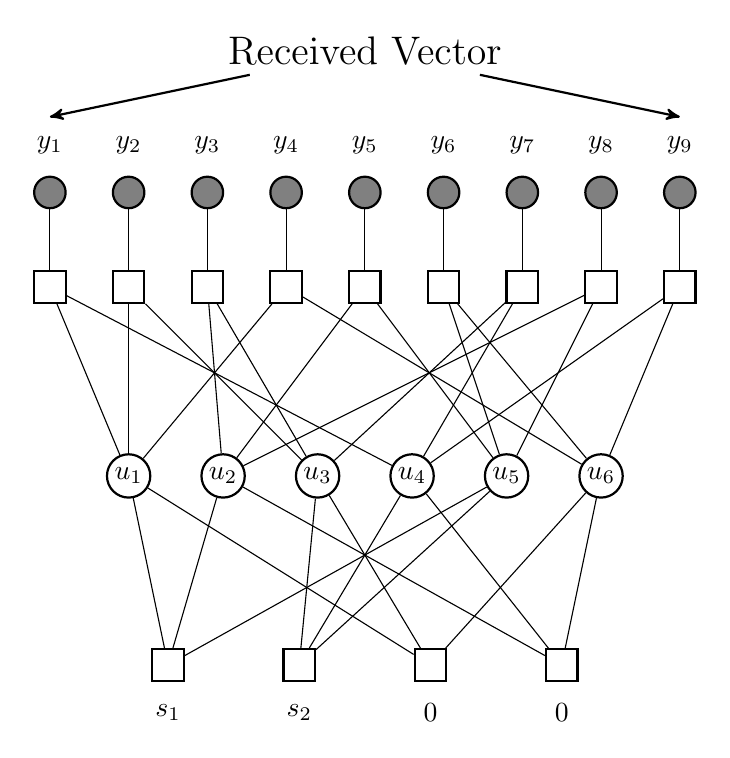
\begin{tikzpicture}
  [
  yscale=1.2,
  node distance = 12mm, draw=black, thick, >=stealth',
  bitnode/.style={circle, inner sep = 0pt, minimum size = 5.5mm, draw=black},
  checknode/.style={rectangle, inner sep = 0pt, minimum size = 4mm, draw=black},
  bitnode2/.style={circle, inner sep = 0pt, minimum size = 4mm, draw=black, fill=black!50},
  ]
  
  \node (rv) at (0,4.5) {\Large{Received Vector}};
  \draw[->] (rv) -- (-4,3.8);
  \draw[->] (rv) -- (4,3.8);

  \foreach \x in {1,2,...,9} {
    \node[bitnode2] (bb\x) at (\x-5,3) {};
  }

  \foreach \x in {1,2,...,9} {
    \node at (\x-5,3.5) {$y_{\x}$};
  }

  \foreach \x in {1,2,...,9} {
    \node[checknode] (c\x) at (\x-5,2) {};
    \draw[thin] (c\x) -- (bb\x);
  }

  \foreach \x in {1,2,...,6} {
    \node[bitnode] (b\x) at (1.2*\x-4.2,0) {$u_{\x}$};
  }

  \foreach \x in {1,...,4} {
    \node[checknode] (cc\x) at (5*\x/3-2.5-5/3,-2) {};
  }

  \draw[thin] (c1) -- (b4);
  \draw[thin] (c1) -- (b1);
  \draw[thin] (c2) -- (b1);
  \draw[thin] (c2) -- (b3);
  \draw[thin] (c3) -- (b3);
  \draw[thin] (c3) -- (b2);
  \draw[thin] (c4) -- (b1);
  \draw[thin] (c4) -- (b6);
  \draw[thin] (c5) -- (b2);
  \draw[thin] (c5) -- (b5);
  \draw[thin] (c6) -- (b5);
  \draw[thin] (c6) -- (b6);
  \draw[thin] (c7) -- (b3);
  \draw[thin] (c7) -- (b4);
  \draw[thin] (c8) -- (b5);
  \draw[thin] (c8) -- (b2);
  \draw[thin] (c9) -- (b4);
  \draw[thin] (c9) -- (b6);


  \draw[thin] (cc1) -- (b2);
  \draw[thin] (cc1) -- (b1);
  \draw[thin] (cc1) -- (b5);
  \draw[thin] (cc2) -- (b5);
  \draw[thin] (cc2) -- (b3);
  \draw[thin] (cc2) -- (b4);
  \draw[thin] (cc3) -- (b1);
  \draw[thin] (cc3) -- (b3);
  \draw[thin] (cc3) -- (b6);
  \draw[thin] (cc4) -- (b2);
  \draw[thin] (cc4) -- (b6);
  \draw[thin] (cc4) -- (b4);

  \node at (5*1/3-2.5-5/3,-2.5) {$s_1$};
  \node at (5*2/3-2.5-5/3,-2.5) {$s_2$};
  \node at (5*3/3-2.5-5/3,-2.5) {$0$};
  \node at (5*4/3-2.5-5/3,-2.5) {$0$};
\end{tikzpicture}

%%% Local Variables: 
%%% mode: latex
%%% TeX-master: "../talk"
%%% End: 
}

    \column{0.5\textwidth}
    \scalebox{0.5}{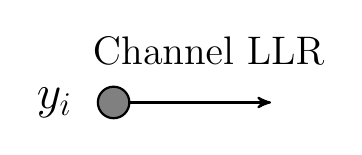
\begin{tikzpicture}
  [
  yscale=1.2,
  node distance = 12mm, draw=black, thick, >=stealth',
  bitnode/.style={circle, inner sep = 0pt, minimum size = 5.5mm, draw=black},
  checknode/.style={rectangle, inner sep = 0pt, minimum size = 4mm, draw=black},
  bitnode2/.style={circle, inner sep = 0pt, minimum size = 4mm, draw=black, fill=black!50},
  ]

  \node at (-0.75,0) {\LARGE{$y_i$}};
  \node[bitnode2] (vv1) at (0,0) {};
  
  \draw[->] (vv1) -- node[above,xshift=0.1cm,yshift=0.35cm]{\Large{Channel LLR}} (2,0);

\end{tikzpicture}


%%% Local Variables: 
%%% mode: latex
%%% TeX-master: "../talk"
%%% End: 
}\\ \vspace{0.3cm}
    \scalebox{0.5}{\input{Figures/mp_ldpc_bit}}\\ \vspace{0.3cm}
    \scalebox{0.5}{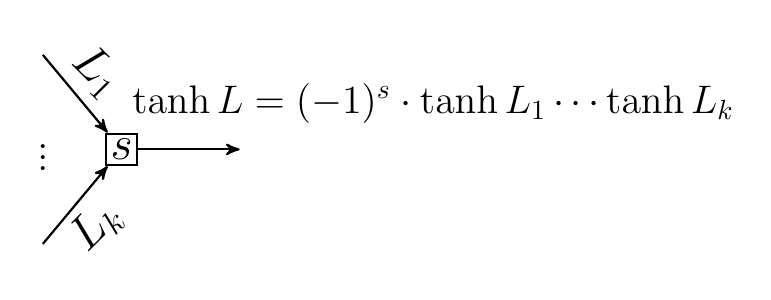
\begin{tikzpicture}
  [
  yscale=1.2,
  node distance = 12mm, draw=black, thick, >=stealth',
  bitnode/.style={circle, inner sep = 0pt, minimum size = 5.5mm, draw=black},
  checknode/.style={rectangle, inner sep = 0pt, minimum size = 4mm, draw=black},
  bitnode2/.style={circle, inner sep = 0pt, minimum size = 4mm, draw=black, fill=black!50},
  ]

  \node[checknode] (v1) at (0,0) {\LARGE{$s$}};
  
  \draw[->] (-1,1) -- node[midway,above,sloped]{\LARGE{$L_1$}} (v1);
  \node at (-1,0) {\LARGE{$\vdots$}};
  \draw[->] (-1,-1) -- node[midway,below,sloped]{\LARGE{$L_k$}} (v1);

  \draw[->] (v1) -- node[above,midway,xshift=3.1cm,yshift=0.2cm]{\Large{$\tanh L=(-1)^{s}\cdot \tanh L_1\cdots \tanh L_k$}} (1.5,0);

\end{tikzpicture}

%%% Local Variables: 
%%% mode: latex
%%% TeX-master: "../talk"
%%% End: 
}
  \end{columns}
  \begin{block}{Remarks}
    \begin{itemize}
    \item Standard message-passing algorithm
    \item Threshold saturation proven for SC compound codes on BEC
    \item Empirically observed for BMS channels
    \end{itemize}
  \end{block}
\end{frame}

\begin{frame}{Numerical Results: Noiseless WOM}
\begin{center}
\begin{tabular}{|c|c|c|c|c|}
\hline
LDGM/LDPC & $\delta^{*}$ & $\delta$ & $\delta$ & $\delta$ \\
$(d_v,d_c,d'_v,d'_c)$ & & $w=2$ & $w=3$ & $w=4$ \\
\hline
$(3,3,3,6)$  & $0.500$ & $0.477$ & $0.492$ & $0.494$\\
$(3,3,4,6)$  & $0.333$ & $0.294$ & $0.324$ & $0.326$\\
$(3,3,5,6)$  & $0.167$ & $0.095$ & $0.156$ & $0.158$\\
$(4,4,3,6)$  & $0.500$ & $0.461$ & $0.491$ & $0.492$\\
$(4,4,4,6)$  & $0.333$ & $0.278$ & $0.323$ & $0.325$\\
$(4,4,5,6)$  & $0.167$ & $0.086$ & $0.155$ & $0.159$\\
$(5,5,3,6)$  & $0.500$ & $0.436$ & $0.488$ & $0.491$\\
$(5,5,4,6)$  & $0.333$ & $0.260$ & $0.320$ & $0.324$\\
$(5,5,5,6)$  & $0.167$ & $0.079$ & $0.154$ & $0.159$\\
\hline  
\end{tabular}
\end{center}
\begin{block}{Remarks}
  \begin{itemize}
  \item $\delta^*$ is the Shannon threshold
  \item $L=30$, Single system length $\approx 24000$
  \end{itemize}
\end{block}
\end{frame}

\begin{frame}{Numerical Results: WOM with Read Errors}
  \begin{center}
    \begin{tabular}{|c|c|c|c|}
      \hline
      LDGM/LDPC & $w$ & $(\delta^{*},p^*)$ & $(\delta,p)$ \\
      $(d_v,d_c,d'_v,d'_c)$ &  &  & \\
      \hline
      $(3,3,4,6)$ & $3$ & $(0.333,0.0615)$ & $(0.321,0.0585)$ \\
      $(3,3,4,8)$ & $3$ & $(0.500,0.0417)$ & $(0.490,0.0387)$ \\
      $(3,3,6,8)$ & $4$ & $(0.250,0.0724)$ & $(0.239,0.0684)$ \\
      $(4,4,4,6)$ & $4$ & $(0.333,0.0615)$ & $(0.324,0.0585)$ \\
      $(4,4,4,8)$ & $4$ & $(0.500,0.0417)$ & $(0.492,0.0387)$ \\
      $(4,4,6,8)$ & $4$ & $(0.250,0.0724)$ & $(0.241,0.0694)$ \\
      \hline  
    \end{tabular}
  \end{center}
  \begin{block}{Remarks}
    \begin{itemize}
    \item $\delta^*$ and $p^*$ are the Shannon thresholds
    \item $L=30$, Single system length $\approx 30000$
    \end{itemize}
  \end{block}
\end{frame}

\begin{frame}{Numerical Results: Small Blocklength}
\begin{figure}[!tbh]
  \centering
  \setlength\tikzheight{3cm}
  \setlength\tikzwidth{6cm} 
  % This file was created by matlab2tikz v0.1.2.
% Copyright (c) 2008--2011, Nico Schlömer <nico.schloemer@gmail.com>
% All rights reserved.
% 
% The latest updates can be retrieved from
%   http://www.mathworks.com/matlabcentral/fileexchange/22022-matlab2tikz
% where you can also make suggestions and rate matlab2tikz.
% 
\begin{tikzpicture}

\begin{semilogyaxis}[%
scale only axis,
width=\tikzwidth,
height=\tikzheight,
xmin=0.38, xmax=0.47,
ymin=1e-05, ymax=1,
xlabel={The normalized weight after first write $\delta$},
ylabel={Encoding failure probability},
xmajorgrids,
ymajorgrids]

\addplot [
line width=1.5pt,
color=blue,
solid,
]
coordinates{
 (0.42,0)(0.43,9e-05)(0.44,0.00337)(0.45,0.07987)(0.46,0.5318)(0.47,0.9654) 
};

\end{semilogyaxis}
\end{tikzpicture}


%%% Local Variables: 
%%% mode: latex
%%% TeX-master: "../paper"
%%% End: 

\end{figure}
\begin{block}{Remarks}
  \begin{itemize}
  \item $(L,w)=(30,3)$, Single system length $1200$, Shannon threshold of $0.5$
  \item A total of $10^5$ were attempted to encode
  \item No failures for $\delta < 0.43$
  \end{itemize}
\end{block}
\end{frame}

\begin{frame}{Concluding Remarks}
  \begin{block}{Conclusion}
    \begin{itemize}
    \item Spatially-coupled compound codes achieve the capacity of 2-write systems \vspace{0.2cm}
    \item \textcolor{red}{Coupling structure} is also crucial 
      \begin{itemize}
      \item to achieve optimum thresholds  
      \item for encoding to succeed 
      \end{itemize}
    \end{itemize}
  \end{block}
  \begin{block}{Multi-Write Systems}
    \begin{itemize}
    \item Will BPGD work for multi-write systems?
    \end{itemize}
  \end{block}
\end{frame}

\end{document}
